\section{Hardware}
This section will describe and compare hardware that can be used to satisfy the requirements of the project.

\subsection{Specifications for NXT}

\begin{figure}[hbtp]
\centering
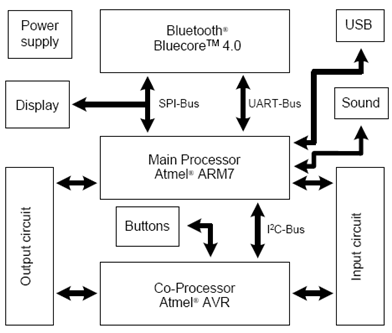
\includegraphics[width=.7\textwidth]{img/lego-nxt-overview.png}
\caption{Overview of the LEGO NXT\cite{nxtspec}.} 
\label{fig:nxt-overview} 
\end{figure}

The LEGO Mindstorms NXT programmable robotics kit consists of various sensors, and a small computer which shall henceforth be called the NXT. \autoref{fig:nxt-overview} shows the internals of the NXT. Within the NXT is an ARM7 32-bit processor with 256kb of flash memory and 64kb of RAM. There is also an 8-bit AVR microcontroller with 4kb of flash memory and 512 bytes of RAM\cite{nxtspec}. The ARM CPU is used for general computations, while the AVR microcontroller is used to control the sensors and servo motors that can be connected to the NXT. The NXT also has a small LCD screen, Bluetooth support, a speaker, and can be connected to a computer through USB. It can take input from four sensors and control three motors at a time.

\subsubsection{ARM CPU}
The ARM family of chipsets are designed using the reduced instruction set computing (RISC) principles\cite{armarchitecture}. RISC processors generally use a small but optimized instruction set, and use the load/store architecture, which only allows memory to be accessed by load and store operations. ARM7 processors have a three stage pipeline. ARM processors differ from the regular x86 processors used in most personal computers in many ways. The shorter pipeline and smaller instruction set makes ARM processors much easier to predict, and because of this it is also possible to optimize software for ARM processors much better than for x86 processors.

ARM processors are usually used in embedded systems such as cell phones, TVs, and most other consumer electronics. The reason for the ARM processors widespread use, is a relatively high performance at a low power consumption and a low price.\cite{armarchitecture}

\subsubsection{Sensors}
The NXT can be connected to many different sensors, which provide different ways of controlling the NXT.
The NXT sensors are as follows\cite{nxtspec}:

\begin{itemize}
\item {Touch sensors}\\ These are simple on/off switches that report if they are pressed or not.
\item {Sound sensors} \\ These can measure sound up to 90 dB.
\item {Light sensors} \\ Light sensors can measure light intensity in a room and on colored surfaces.
\item {Color sensors} \\ These further developed light sensors, that can detect six different colors as well as the light intensity in a room.
\item {Ultrasonic sensors} \\ These can be used to see and recognize objects, measure distances and detect movement. They work by sending out ultrasonic sound waves that bounce off objects and are sent back. By measuring the time it takes for the sound waves to come back, the sensor can calculate the distance to the object. The object has to have a flat surface for the ultrasonic sensor to detect it.
\item {Infrared sensors} \\ Like the ultrasound sensors these can measure distance but instead of sound they use an infrared light emitter, and like the ultrasound sensor measure the time it takes for the light to bounce off an object and return.
\item {Servo motors} \\ Servo motors can rotate and move objects. Furthermore they have a built-in rotation sensor to allow them to be used as sensors as well as actuators. The NXT can also control the speed of the servo motors.
\item {Infrared obstacle detector} \\ These can detect an obstacle in six different zones.
\end{itemize}

The sensors that are most relevant for the project, are the servo motors to rotate the turret, the ultrasonic sensor, the infrared obstacle detector and the touch sensors.

\subsection{Specifications for Kinect}

\begin{figure}[hbtp]
\centering
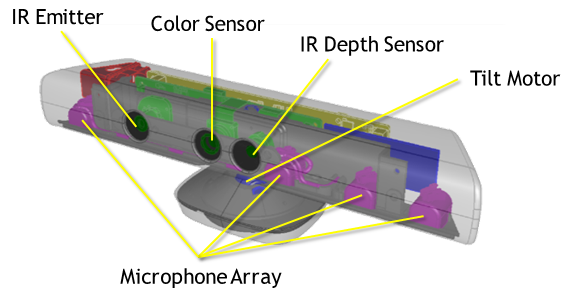
\includegraphics[width=.7\textwidth]{img/kinect-overview.png}
\caption{Overview of the Kinect\cite{kinectspec}.} 
\label{fig:kinect-overview} 
\end{figure}

An alternative to the ultrasound sensor is the Kinect from Microsoft. The Kinect is developed for the Xbox 360 to facilitate input without a typical controller. Instead the input is body movement from a person standing in front of the Kinect. \autoref{fig:kinect-overview} shows the Kinect which registers body movement by using a RGB camera and an Infrared (IR) Depth Sensor\cite{kinectspec}. The regular RGB camera creates color images with up to 1280x960 pixel resolution. The IR Depth Sensor works in combination with an IR Emitter that emits infrared light beams. The IR Depth Sensor reads these beams as they are reflected back from an object, measuring the distance between the object and the sensor. Both the RGB camera and the IR Depth Sensor have a 30 Hz refresh rate. The field of view for the Kinect is 57 degrees horizontally and 34 degrees vertically.

Even though the Kinect was designed to be used by the Xbox 360, an SDK for Windows has been released, which allows the Kinect to be connected to a PC instead of an Xbox. The Kinect is thus capable of much more than finding people and their movements.

\subsection{LEGO Technic Competition Cannon}

\begin{figure}[hptb]
  \centering
    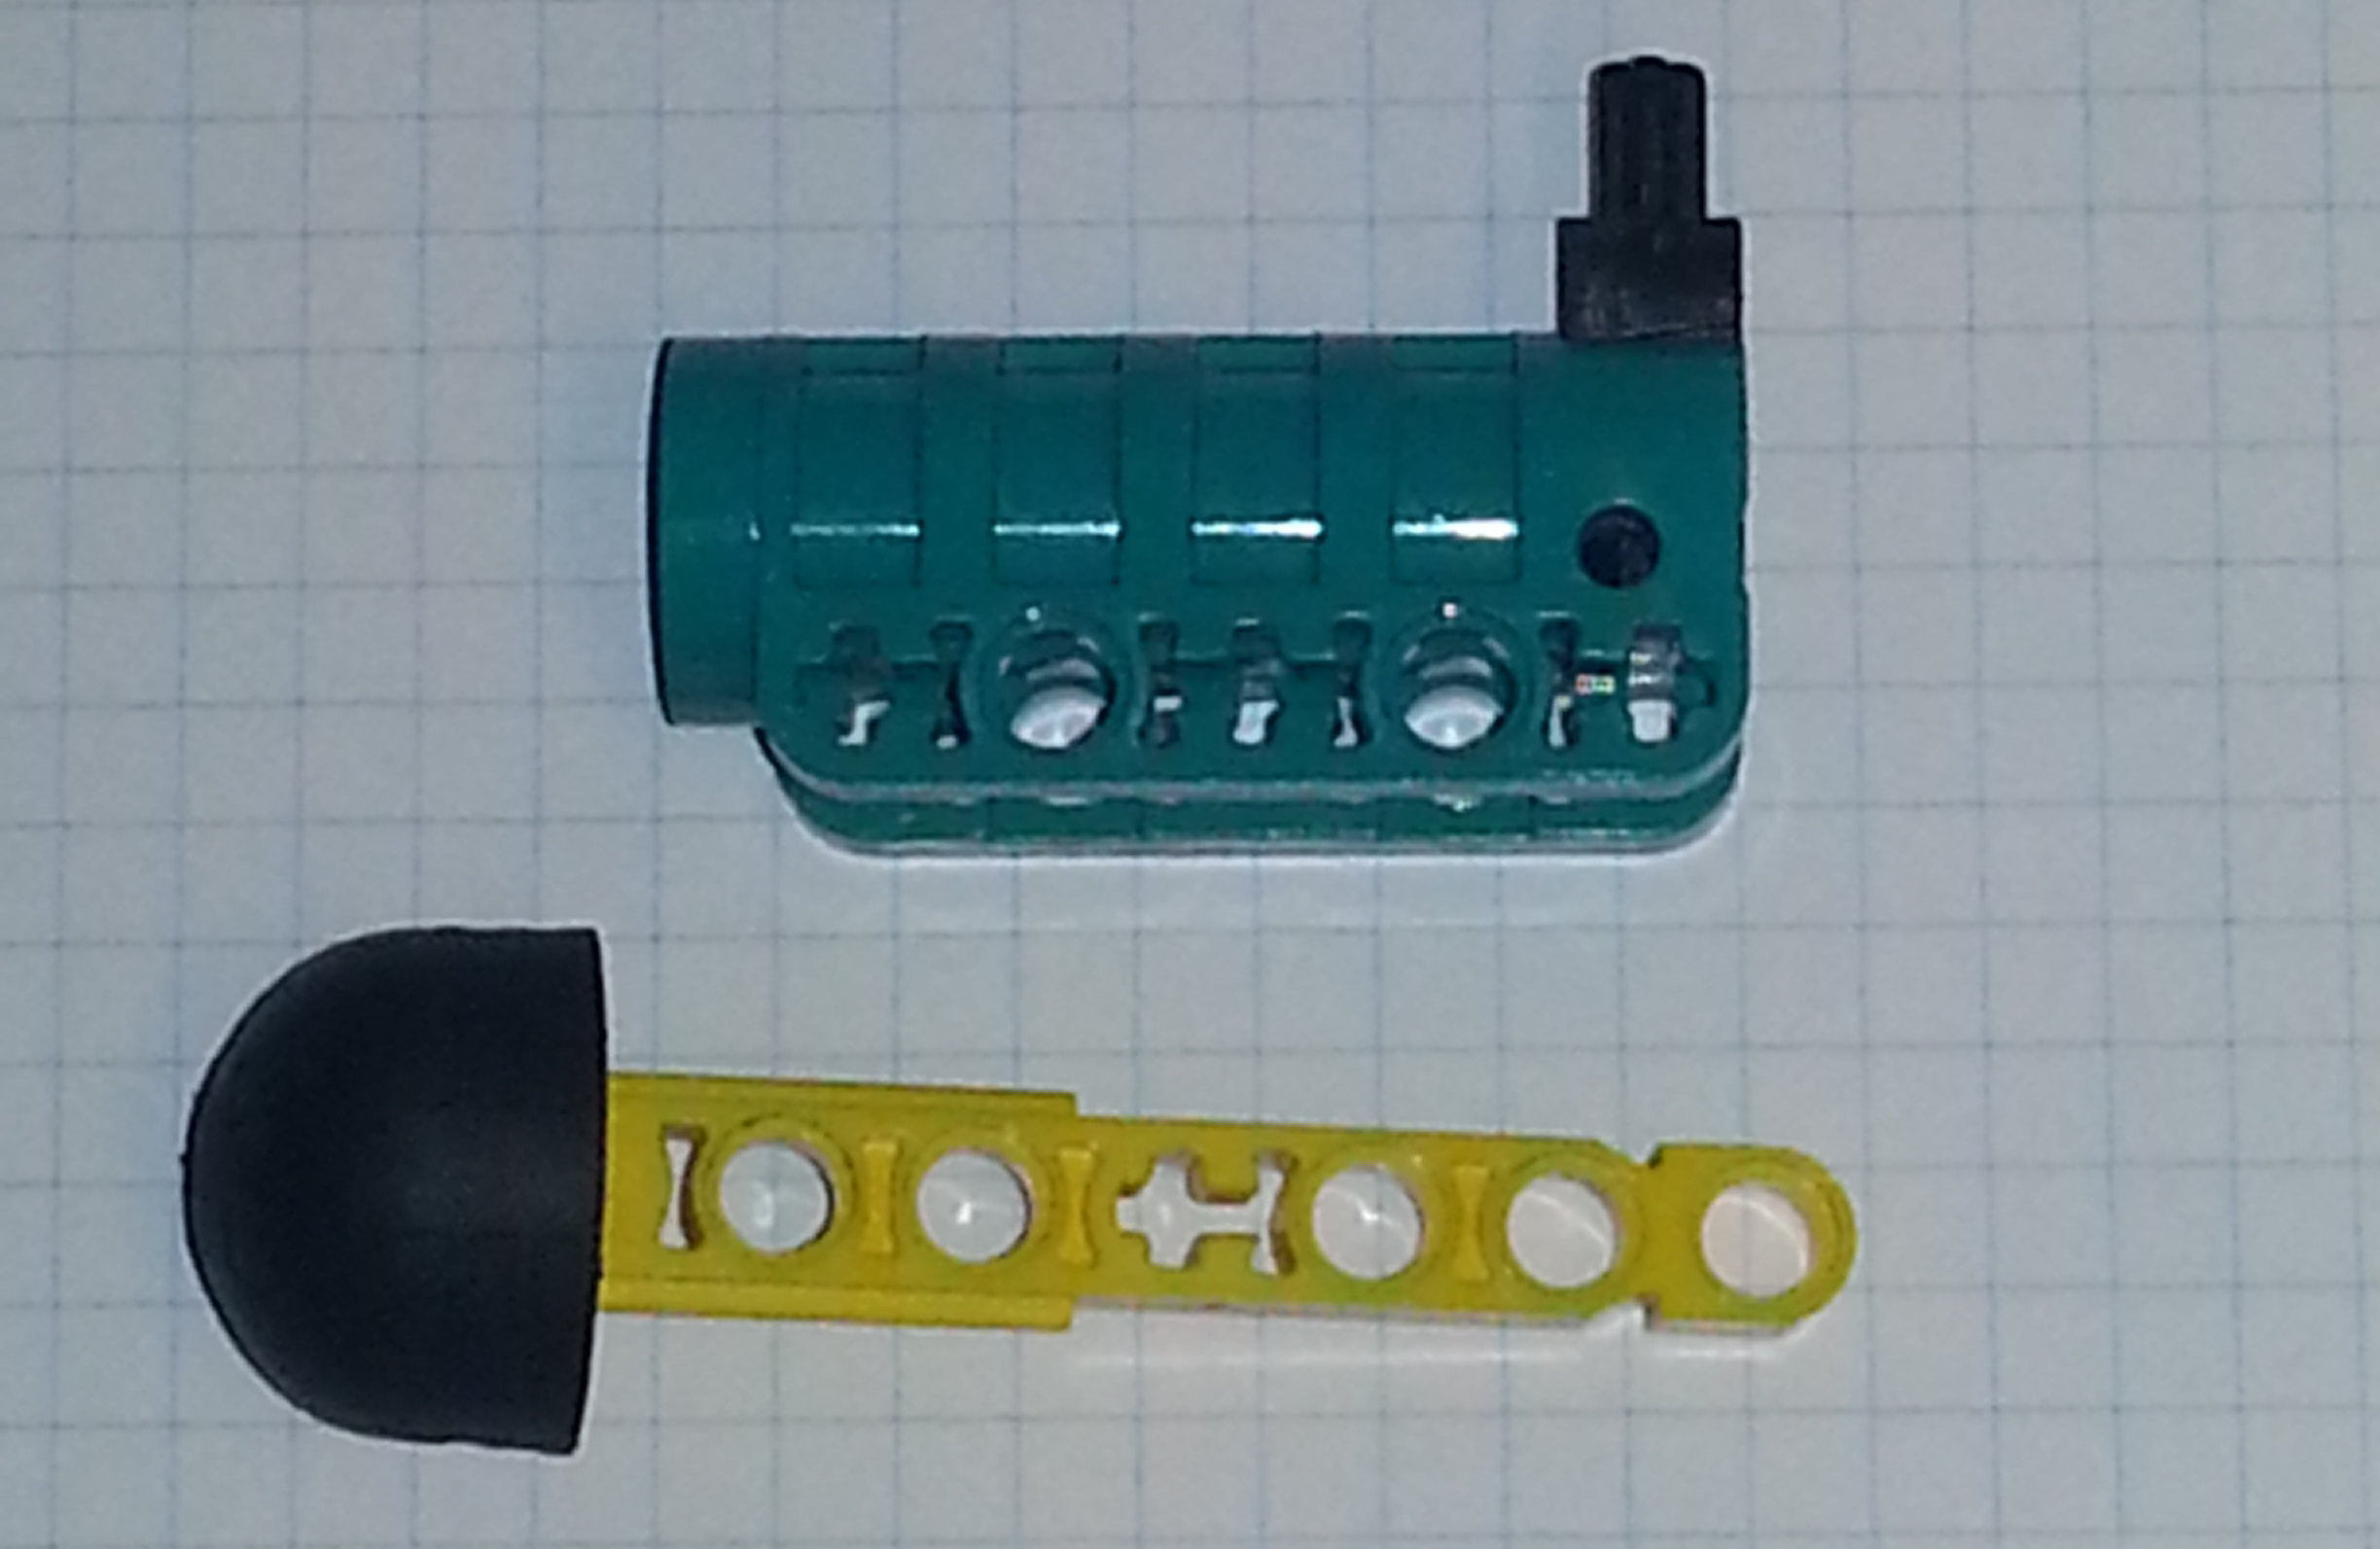
\includegraphics[width=0.5\textwidth]{img/competition_cannon.png}
  \caption{Our projectile firing mechanism}
  \label{competition_cannon}
\end{figure}

LEGO provides the Competition Cannon, a spring-powered cannon that fits the LEGO that will be used to build the turret, while being able to produce reasonably precise and consistent shots.

\subsection{Preliminary tests}
To find the correct hardware to use, it is necessary to have information to make the correct decision. These tests include a comparison between the Kinect and the LEGO ultrasound sensor, and measurements of the precision of the LEGO Competition Cannon.

\subsubsection{Kinect \& LEGO ultrasound sensor}
When testing the Kinect and ultrasound sensor precision, the distance to an object was measured with a tape measure, and compared it to the distance reported from the sensors.

\autoref{fig:kinect-distance} shows the results from the Kinect testing, and \autoref{fig:ultrasound-distance} shows the result from the ultrasound sensor test.

\begin{figure}[hbtp]
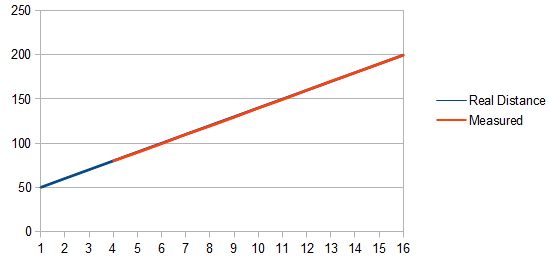
\includegraphics[width=\textwidth]{img/kinect-distance.png}
\caption{Kinect distance measurement.} 
\label{fig:kinect-distance} 
\end{figure}

\begin{figure}[hbtp]
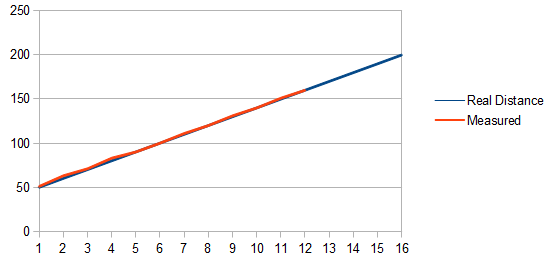
\includegraphics[width=\textwidth]{img/ultrasound-distance.png}
\caption{Ultrasound distance measurement.} 
\label{fig:ultrasound-distance} 
\end{figure}

The tests show that while the ultrasound sensor is a bit unprecise between 50 and 80 cm, the Kinect cannot measure closer than 80 cm, thus giving the ultrasound sensor an advantage.
On the other side of the spectrum, however, the ultrasound sensor cannot measure above 160 cm, while the Kinect can measure precisely at least up to a maximum distance measured of 200 cm.
Generally, the precision of both the ultrasound sensor and the Kinect is precise down to \textpm1 cm between 80 and 160 cm. The Kinect retains this precision up to at least 200 cm.

Where the Kinect has a field of view that objects can enter, the ultrasound sensor can only measure the distance of an object straight in front of the sensor. The ultrasound sensor needs the help of another sensor to be able to do what the Kinect can do out of the box. Using a webcam in combination with the ultrasound sensor, could come close in functionality to the Kinect. Another option is to use a the infrared obstacle detector instead of a webcam in combination with the ultrasound sensor, but this option will be limited in functionality compared to the webcam or Kinect solution, as the infrared obstacle detector only has six zones of detection.

\subsection{Range of Cannon}
\label{cannonrange}
The cannon's range has been measured by repeatedly shooting the cannon from specific angles, and calculating the average travel distance of the projectile. \autoref{fig:cannon-range} shows the average ranges from the measured angles.

These tests have been performed with the cannon at 80 cm above the ground.

\begin{figure}[hbtp]
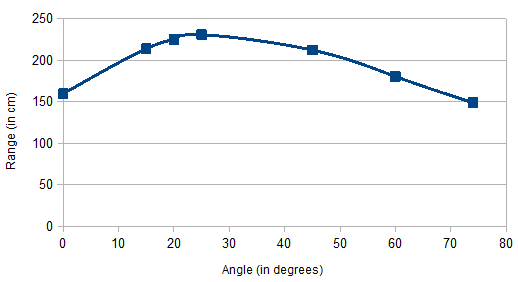
\includegraphics[width=\textwidth]{img/cannon-range.png}
\caption{The range of the cannon.} 
\label{fig:cannon-range} 
\end{figure}

It can be gathered from \autoref{fig:cannon-range} that the cannon shoots furthest at a 25 degree angle, where it shot the projectile a distance of 230 cm and that shooting from 0 degrees gives the same result of 160 cm as shooting from 65 degrees. The results of the shots vary with a few centimeters in each direction from the average.

\subsection{Projectile Speed}
To measure the speed of the projectile, three videos of the projectile firing in front of lines with 10 cm between them were taken. The videos were then framed through to calculate the speed. \autoref{tab:projectile-speed} shows the results of our calculations.

\begin{table}[htbp]
\begin{tabular}{|p{4cm}|p{4cm}|p{4cm}|}
\hline
\textbf{Test 1} & \textbf{Test 2} & \textbf{Test 3} \\
\hline
450 cm/s & 428 cm/s & 450 cm/s\\
\hline
$\sim$ 60 cm in 4 frames & $\sim$ 100 cm in 7 frames & $\sim$ 60 cm in 4 frames \\
\hline
\end{tabular}
\caption{Initial speed of the projectile}
\label{tab:projectile-speed}
\end{table}

These calculations show, that the cannon can hit any target closer than 2 meters in less than half a second. The speed measured is the initial speed and friction is ignored.